\documentclass[conference]{IEEEtran}
\IEEEoverridecommandlockouts

\usepackage{cite}
\usepackage{amsmath,amssymb,amsfonts}
\usepackage{algorithmic}
\usepackage{graphicx}
\usepackage{textcomp}
\usepackage{xcolor}
\usepackage{booktabs}
\usepackage{multirow}
\usepackage{url}
\usepackage{listings}
\usepackage{hyperref}
\usepackage{balance}
\usepackage{tikz}
\usepackage{pgfplots}
\pgfplotsset{compat=1.18}
\usetikzlibrary{shapes.geometric, arrows.meta, positioning, fit, backgrounds, calc}

\lstset{
  basicstyle=\ttfamily\footnotesize,
  breaklines=true,
  frame=single,
  numbers=left,
  numberstyle=\tiny,
  tabsize=2
}

\def\BibTeX{{\rm B\kern-.05em{\sc i\kern-.025em b}\kern-.08em
    T\kern-.1667em\lower.7ex\hbox{E}\kern-.125emX}}

\begin{document}

\title{Performance Evaluation of Blockchain-Based Security Logging for Advanced Air Mobility Systems}

\author{
\IEEEauthorblockN{Daniel Garcia}
\IEEEauthorblockA{
\textit{Department of Computer Engineering} \\
\textit{Polytechnique Montreal}\\
Montreal, Canada \\
daniel.garcia@polymtl.ca}
}

\maketitle

\begin{abstract}
Advanced Air Mobility (AAM) systems face cybersecurity challenges requiring tamper-evident logging of security events such as GPS spoofing and denial of service attacks. The multi-stakeholder nature of AAM---involving operators, regulators, and insurers---creates trust requirements where no single party should control audit logs. Blockchain has been proposed for distributed, immutable logging, but its performance overhead remains unquantified for AAM. This paper presents an empirical evaluation comparing PostgreSQL with hash-chained audit logs, Hyperledger Fabric (permissioned blockchain), and Solana (public blockchain) for security event logging. Using real UAV cyberattack datasets containing 157,501 events across six attack types, we measured latency, throughput, and security guarantees. Results show PostgreSQL achieves 1.39ms P95 latency at 5,000 TPS, compared to 2,182ms for Hyperledger Fabric (22x slower) and 15,157ms for Solana (152x slower). All systems passed tamper detection tests. We conclude that blockchain cannot meet real-time alerting requirements (<100ms) but remains viable for audit trail logging when multi-party verification is required. A hybrid architecture combining PostgreSQL for real-time operations with periodic blockchain anchoring provides optimal balance of performance and distributed trust.
\end{abstract}

\begin{IEEEkeywords}
blockchain, advanced air mobility, cybersecurity, Hyperledger Fabric, Solana, performance evaluation, UAV security, audit logging, eVTOL, GPS spoofing
\end{IEEEkeywords}

\section{Introduction}

Urban Air Mobility (UAM) represents a paradigm shift in transportation, with electric aircraft designed to carry passengers through urban airspace. Companies including Joby Aviation, Lilium, and Archer are developing eVTOL aircraft with projected commercial operations by 2025 \cite{straubinger2020}. The global UAM market is projected to reach \$15 billion by 2030, with thousands of aircraft operating in metropolitan areas \cite{pak2024}. These systems rely on digital command and control (C2) links, GPS navigation, and networked communication that create attack surfaces similar to traditional UAV systems.

The cybersecurity requirements for AAM differ fundamentally from those of ground vehicles or enterprise IT systems. Aircraft operate under strict latency constraints where delayed attack detection can result in loss of life. The FAA and EASA have established certification requirements that mandate auditable security logging \cite{faa2023}. The JARUS (Joint Authorities for Rulemaking of Unmanned Systems) has published Required Communication Performance (RCP) specifications that define latency thresholds for safety-critical aviation communications \cite{jarus2023}. Simultaneously, the multi-stakeholder nature of urban airspace---involving operators, regulators, vertiport managers, and insurance providers---creates trust requirements that centralized databases cannot satisfy.

The multi-stakeholder nature of AAM operations creates a fundamental trust problem that motivates blockchain consideration. When a security incident occurs---such as GPS spoofing causing a near-collision---multiple parties require access to tamper-evident logs: the aircraft operator for internal review, aviation regulators (FAA, EASA) for compliance verification, insurance companies for claims processing, and potentially law enforcement for investigation. A centralized database controlled by any single party cannot provide the independent verifiability that all stakeholders require. The operator could theoretically modify logs to minimize liability; regulators cannot trust records they do not control; insurers need cryptographic proof that records existed at the time of the incident.

Blockchain technology addresses this trust gap through distributed consensus \cite{reisman2019}. By replicating the security event log across multiple independent nodes operated by different stakeholders, blockchain ensures that no single party can unilaterally modify historical records. The cryptographic linking of blocks provides tamper-evidence: any modification to past entries invalidates subsequent hashes, making tampering detectable. This architectural property is essential for regulatory compliance and incident investigation in safety-critical aviation systems.

However, blockchain consensus mechanisms inherently introduce latency that may conflict with real-time requirements. Previous research has examined blockchain for UTM (Unmanned Traffic Management) operational intent registration \cite{permissioned2024} but has not quantified the performance overhead for security event logging specifically. This gap motivates our empirical evaluation: we need to determine whether blockchain's trust benefits justify its performance costs for AAM security logging.

This paper addresses three research questions:

\begin{itemize}
\item \textbf{RQ1}: Can blockchain meet AAM real-time alert requirements (P95 latency < 100ms)?
\item \textbf{RQ2}: What is the maximum throughput each system can sustain before performance degradation?
\item \textbf{RQ3}: Does blockchain provide security guarantees that justify its performance overhead compared to hash-chained databases?
\end{itemize}

We implemented security logging systems across PostgreSQL, Hyperledger Fabric, and Solana, then conducted controlled experiments using real UAV attack datasets. Our contributions include:

\begin{itemize}
\item First quantitative comparison of blockchain versus traditional databases for AAM security event logging using real attack data
\item Open-source implementations of security logging smart contracts for Hyperledger Fabric (Go chaincode) and Solana (Rust/Anchor program)
\item Empirical evidence that blockchain latency exceeds real-time thresholds by 22x--152x
\item A hybrid architecture recommendation balancing real-time performance with immutable audit requirements
\end{itemize}

The remainder of this paper is organized as follows. Section \ref{sec:related} reviews related work on blockchain for aviation security and UAV cybersecurity threats. Section \ref{sec:methodology} describes our methodology including datasets, system implementations, and test procedures. Section \ref{sec:results} presents experimental results. Section \ref{sec:discussion} discusses implications and limitations. Section \ref{sec:conclusion} concludes with recommendations.

\section{Related Work}
\label{sec:related}

\subsection{Cybersecurity Threats in Urban Air Mobility}

The attack surface of AAM systems encompasses multiple vectors that traditional aviation has not confronted. NASA conducted a comprehensive review of cybersecurity vulnerabilities for Urban Air Mobility, identifying GPS spoofing, communication hijacking, and adversarial machine learning as primary concerns \cite{nasa2020}. The review noted that ``while fixed-wing commercial aircraft have a range of back-up systems in case their GPS systems are attacked, this may not be the case with eVTOLs, where sensors may be the only means of navigation.''

GPS spoofing represents a particularly severe threat. Between 2023 and 2025, the Indian government reported over 465 cases of GPS spoofing and interference affecting both surveillance and commercial flights \cite{verticalmag2024}. Nation-states have demonstrated the capability to broadcast false position signals that deceive aircraft navigation systems, potentially causing aircraft to deviate from intended flight paths. As UAVs rely on GPS for positioning and navigation, they can fall prey to GPS jamming and spoofing attacks that redirect victim drones for malicious purposes.

Ajakwe et al. examined security paradigms for smart aerial mobility and intelligent logistics, categorizing attacks into sensor-based (jamming, GPS spoofing), software-based (zero-day, malware, backdoor), and communication-based (man-in-the-middle, replay) categories \cite{ajakwe2024}. Their analysis highlighted that real-time threat detection requires sub-second response times that blockchain systems struggle to achieve.

Hassler et al. developed a cyber-physical intrusion detection dataset for UAVs encompassing de-authentication DoS attacks, replay attacks, false data injection, and evil twin attacks \cite{hassler2023}. Their dataset, which we use in this study, demonstrates that real UAV systems face diverse and sophisticated threats. The dataset was collected from a physical testbed including quadcopters, ground control stations, and monitoring infrastructure, providing realistic attack signatures.

ADS-B (Automatic Dependent Surveillance-Broadcast) presents additional vulnerabilities. Due to ADS-B's unencrypted and unauthenticated nature, possible threats include jamming, denial of service, eavesdropping, spoofing, message injection, and message manipulation \cite{reisman2019}. Security researchers have confirmed that ADS-B spoofing attacks are ``not only possible but easy and practically feasible, for a moderately sophisticated attacker.''

\subsection{Blockchain for Aviation Systems}

Reisman proposed the first blockchain infrastructure for air traffic management at NASA Ames Research Center, using Hyperledger Fabric to address ADS-B spoofing and privacy concerns \cite{reisman2019}. The design separates public aircraft state data from private flight plan information across separate channels. The architecture enables multi-stakeholder verification while preserving operational security. While architecturally sound, the paper did not report performance measurements under load.

Allouch et al. developed UTM-Chain, a Hyperledger Fabric solution for securing UAV flight plans and data records \cite{allouch2021}. They reported transaction latencies and resource utilization via cAdvisor, establishing methodology for blockchain UAV performance evaluation. Their system achieved latencies in the hundreds of milliseconds range for flight plan registration, though security event logging was not specifically addressed.

Most relevant to our work, researchers evaluated permissioned blockchain for AAM operational intent registration using Hyperledger Fabric and the InterUSS Platform \cite{permissioned2024}. Testing across geographically distributed nodes in Brazil (separated by approximately 2,500 km), they found that ``InterUSS sustained sub-second latency up to 30 TPS with stable tails, while Fabric exceeded 3 second median latency and 15 second p90 beyond this load, saturating near 50 TPS.'' The study concluded that ``current permissioned-ledger designs cannot meet aeronautical real-time constraints'' and recommended a hybrid model coupling federated coordination with DLT-based auditability.

Freeman et al. at NASA examined blockchain for UAM operational intent data exchange, validating cybersecurity benefits but identifying consensus optimization needs for real-time constraints \cite{freeman2023}. Their case study demonstrated that permissioned blockchain with identified organizations provides audit trails satisfying FAA/EASA requirements.

Hossain et al. conducted a comprehensive analysis of blockchain integration in UAV networks, examining performance metrics including throughput, latency, scalability, and packet size \cite{hossain2024}. Their reputation-based consensus mechanism achieved 94\% trust score prediction accuracy and 96\% rogue UAV detection rate. However, they noted that ``the UAV swarm network experiences a large computational delay due to blockchain security procedures, making it inappropriate for applications that need low latency and high availability.''

The SkyTrust framework proposed an energy-aware consensus protocol in Hyperledger Fabric specifically for UAV applications \cite{skytrust2024}. Simulation results showed the framework outperformed centralized and static baselines on privacy, energy efficiency, and reliability, though latency remained above real-time thresholds.

\subsection{Blockchain Performance Characteristics}

Solana represents the highest-throughput public blockchain, advertising sub-second block times and theoretical TPS exceeding 50,000 \cite{solana2024}. However, research demonstrates significant nuances in these claims. The Crypto Research Report analyzed Solana finality, finding that ``block finality is currently 12.8 seconds, with optimistic confirmations at about 500 to 600 milliseconds'' \cite{cryptoresearch2024}. Full finalization requires approximately 32 slots at 400ms each, totaling 12.8 seconds under normal conditions.

Solana's network performance has shown improvement but also vulnerabilities. The March 2024 Network Performance Report documented a 4 hour 46 minute outage on February 6, 2024, caused by a bug in the LoadedPrograms function that led to an infinite loop and halted consensus \cite{solana_perf2024}. For safety-critical aviation applications, such reliability concerns are significant.

The upcoming Alpenglow protocol promises to reduce Solana's finality from 12.8 seconds to under 250ms (median approximately 150ms), representing a potential 100x improvement \cite{alpenglow2024}. However, this upgrade was not available during our experiments, and production deployment timelines remain uncertain.

Hyperledger Fabric performance depends heavily on network configuration. Comprehensive benchmarking by the Hyperledger Foundation across more than 1,500 network configurations and 200 million transactions found that ``as long as the transaction rate is maintained within 200 transactions per second, the network latency is in the order of fraction of a second'' \cite{hyperledger2023}. Beyond this threshold, latency increases exponentially due to ordering service bottlenecks.

Sukhwani et al. developed analytical models for Hyperledger Fabric latency, identifying endorsement policy, block size, and network topology as primary factors \cite{sukhwani2024}. Their model predicted latency degradation patterns consistent with our experimental observations.

Traditional relational databases like PostgreSQL achieve latencies under 5ms for simple inserts with throughput exceeding 50,000 TPS on commodity hardware \cite{postgresql2024}. These numbers establish the baseline against which blockchain overhead must be measured.

\subsection{Tamper-Evident Logging}

Hash-chained audit logs provide tamper evidence without blockchain overhead. Crosby and Wallach developed efficient data structures for tamper-evident logging using authenticated append-only skip lists \cite{crosby2009}. Their approach enables verification that logs have not been modified since creation.

The technology relies on consecutively hashing all incoming audit log events, where each subsequent hash is formed by the data of the current entry combined with the hash of the previous entry \cite{cossacklabs2024}. This creates a cryptographic chain that cannot be ``broken''---any manipulation to any entry results in invalid hashes from that point forward.

Modern implementations combine PostgreSQL audit logging (via pgaudit) with immutable databases like immudb to create tamper-proof audit trails \cite{codenotary2024}. immudb uses cryptographic hashing and Merkle trees to ensure data integrity, with each record cryptographically linked to its predecessor.

The key distinction between hash-chained databases and blockchain is trust model. Hash chains detect tampering but require trust in the database administrator who controls the system. Blockchain distributes trust across multiple parties through consensus, eliminating single points of compromise at the cost of increased latency.

\section{Methodology}
\label{sec:methodology}

\subsection{Datasets}

We utilized the Cyber-Physical Dataset for UAVs Under Normal Operations and Cyberattacks, published by Hassler et al. through IEEE DataPort \cite{hassler2023}. This dataset is directly applicable to AAM security logging because UAVs and eVTOLs share fundamental attack surfaces: both rely on GPS for navigation, WiFi/cellular links for command and control, and networked communication vulnerable to the same attack vectors. The threat models overlap substantially---GPS spoofing, communication hijacking, and denial of service attacks affect both platforms identically. The dataset was collected from a real UAV testbed including quadcopters, ground control stations, and monitoring infrastructure, providing realistic attack signatures that represent the security events an AAM system would need to log. The work was supported by the National Science Foundation under Award 2220346.

The dataset contains 54,784 records across normal operations and four attack types:
\begin{itemize}
\item \textbf{Benign operations}: Rows 1--13,717 containing cyber and physical telemetry during normal flight operations
\item \textbf{DoS attacks}: Rows 13,718--26,363 capturing de-authentication attacks disrupting the WiFi control link
\item \textbf{Replay attacks}: Rows 26,364--39,344 containing replayed telemetry packets attempting to mask actual vehicle state
\item \textbf{Evil twin attacks}: Rows 39,345--50,502 documenting rogue access point attacks
\end{itemize}

We developed a Rust parser to normalize the raw CSV data into a standardized security event format:

\begin{lstlisting}[language=Rust, caption={Security Event Data Structure}]
struct SecurityEvent {
    timestamp_ms: i64,      // Detection time
    event_type: u8,         // Attack classification
    confidence: u8,         // Detection confidence
    vehicle_id: [u8; 32],   // SHA-256 of vehicle ID
    data_hash: [u8; 32],    // SHA-256 of telemetry
}
\end{lstlisting}

The event\_type field maps attacks: 0=Benign, 1=GPSJam, 2=MITM, 3=Replay, 4=GPSSpoof, 5=DoS, 6=EvilTwin. After processing the original dataset and augmenting with synthetic GPS spoofing, GPS jamming, and MITM attack signatures derived from the CICIoV2024 vehicular intrusion dataset \cite{ciciov2024}, our final dataset contained 157,501 normalized security events. Table \ref{tab:attack_distribution} shows the distribution by attack type.

\begin{table}[htbp]
\caption{Attack Distribution in Processed Dataset}
\label{tab:attack_distribution}
\centering
\begin{tabular}{lrr}
\toprule
\textbf{Attack Type} & \textbf{Count} & \textbf{Percentage} \\
\midrule
Benign & 105,000 & 66.5\% \\
GPS Jamming & 8,848 & 5.6\% \\
MITM & 8,771 & 5.6\% \\
Replay Attack & 8,728 & 5.5\% \\
GPS Spoofing & 8,725 & 5.5\% \\
DoS Attack & 8,724 & 5.5\% \\
Evil Twin & 8,705 & 5.5\% \\
\midrule
\textbf{Total} & \textbf{157,501} & \textbf{100\%} \\
\bottomrule
\end{tabular}
\end{table}

\subsection{System Implementations}

\subsubsection{PostgreSQL with Hash-Chained Audit Log}

We implemented a hash-chained audit table in PostgreSQL 16 that provides tamper-evidence comparable to blockchain. The schema includes:

\begin{lstlisting}[language=SQL, caption={PostgreSQL Schema (excerpt)}]
CREATE TABLE security_events (
    event_id BIGSERIAL PRIMARY KEY,
    event_timestamp TIMESTAMPTZ NOT NULL,
    event_type SMALLINT NOT NULL
        CHECK (event_type BETWEEN 0 AND 6),
    confidence SMALLINT NOT NULL
        CHECK (confidence BETWEEN 0 AND 100),
    vehicle_id BYTEA NOT NULL,
    data_hash BYTEA NOT NULL,
    prev_hash BYTEA NOT NULL,
    record_hash BYTEA NOT NULL,
    created_at TIMESTAMPTZ DEFAULT NOW()
);
\end{lstlisting}

A stored procedure handles insertion while computing hash chains using SHA-256. The \texttt{prev\_hash} field contains the \texttt{record\_hash} of the previous event, creating an unbroken cryptographic chain. A \texttt{verify\_hash\_chain()} function recomputes hashes sequentially to detect any tampering.

The connection pool was configured with 20 persistent connections using asyncpg for Python-based load testing, enabling high-throughput asynchronous operations.

\subsubsection{Hyperledger Fabric}

We deployed Hyperledger Fabric 2.5.10 using the fabric-samples test-network configuration with the following topology:
\begin{itemize}
\item \textbf{Orderers}: 3 Raft consensus nodes (orderer.example.com, orderer2, orderer3) providing crash fault tolerance
\item \textbf{Organizations}: 2 organizations (Org1, Org2) each with one peer node
\item \textbf{Channel}: aamchannel dedicated to security event logging
\item \textbf{StateDB}: LevelDB for key-value state storage
\item \textbf{Endorsement Policy}: AND(Org1.peer, Org2.peer) requiring both organizations
\end{itemize}

Our Go chaincode (439 lines) implements the AAMSecurityContract:

\begin{lstlisting}[language=Go, caption={Hyperledger Chaincode (excerpt)}]
func (c *AAMSecurityContract) LogSecurityEvent(
    ctx contractapi.TransactionContextInterface,
    eventTimestamp int64,
    eventType uint8,
    confidence uint8,
    vehicleID string,
    dataHash string,
) (*SecurityEvent, error) {
    counter, _ := ctx.GetStub().GetState("eventCounter")
    event := SecurityEvent{
        EventID:   counter,
        TxID:      ctx.GetStub().GetTxID(),
        Timestamp: time.Now().Unix(),
        // ... additional fields
    }
    eventJSON, _ := json.Marshal(event)
    ctx.GetStub().PutState(
        fmt.Sprintf("EVENT_%d", counter),
        eventJSON)
    return &event, nil
}
\end{lstlisting}

Transaction flow involves: (1) client submits proposal to endorsing peers, (2) peers execute chaincode and sign results, (3) client collects endorsements and submits to orderer, (4) orderer creates block and distributes to peers, (5) peers validate and commit to ledger.

\subsubsection{Solana}

We deployed a Solana program using Anchor 0.30.1 on a local test validator (Solana CLI 2.2.20). The Rust program stores security events in program-derived accounts:

\begin{lstlisting}[language=Rust, caption={Solana Program (excerpt)}]
#[program]
pub mod aam_security_log {
    pub fn log_security_event(
        ctx: Context<LogEvent>,
        event_timestamp: i64,
        event_type: u8,
        confidence: u8,
        vehicle_id: [u8; 32],
        data_hash: [u8; 32],
    ) -> Result<()> {
        let event = &mut ctx.accounts.event;
        let clock = Clock::get()?;
        event.block_timestamp = clock.unix_timestamp;
        event.slot = clock.slot;
        // ... store fields
        Ok(())
    }
}
\end{lstlisting}

Each event requires creation of a new account, incurring rent-exempt costs of approximately 0.002 SOL on mainnet. The program ID was deployed at \texttt{4KAuuJxmX2x2JD6d3F7jxyUqHNufxkYsaA38Rjbb9Ccr}. We configured the test validator with default settings and waited for transaction confirmation (finalized commitment level) to measure true end-to-end latency.

\subsection{Test Infrastructure}

The complete experimental infrastructure is available as an open-source repository\footnote{\url{https://github.com/danielles0xg/blockchain_on_advanced_aerial_mobility.git}} containing all deployment configurations, smart contracts, and analysis tools. The infrastructure was designed for reproducibility using Infrastructure-as-Code principles.

\subsubsection{Deployment Architecture}
The test environment consists of three isolated deployments:

\textbf{PostgreSQL}: Deployed via Docker Compose with PostgreSQL 16, configured with hash-chaining stored procedures and verification functions. The schema includes indexes on timestamp and event\_type for query optimization.

\textbf{Hyperledger Fabric}: Deployed using the fabric-samples test-network with custom Go chaincode. The network runs three Raft orderers for crash fault tolerance, two peer organizations with endorsement policy requiring both signatures, and LevelDB for state storage. Deployment scripts automate channel creation, chaincode installation, and network initialization.

\textbf{Solana}: Local test validator deployment with custom Anchor program. The Rust program implements account-based event storage with program-derived addresses. Deployment includes keypair generation, program compilation, and validator configuration.

\subsubsection{Test Execution Environment}
All experiments ran on an Apple Silicon M2 Mac (macOS Darwin 23.6.0) with:
\begin{itemize}
\item Docker Desktop 4.x for PostgreSQL and Fabric containers
\item Native Solana test-validator (solana-test-validator 2.2.20)
\item Python 3.13 with asyncpg, solana-py, and solders libraries
\item 20-connection PostgreSQL connection pool
\end{itemize}

\subsubsection{Load Testing Framework}
Our load testing tool (blast.py, 776 lines) implements:
\begin{itemize}
\item Asynchronous event submission with configurable TPS using asyncio
\item Semaphore-based concurrency control (100 for PostgreSQL, 50 for Solana, 20 for Fabric)
\item Real-time latency measurement from submission to confirmation
\item Rate limiting to achieve precise target TPS
\item CSV output for statistical analysis
\end{itemize}

The repository structure organizes code by component: \texttt{blockchain/solana/} for Anchor programs, \texttt{blockchain/hyperledger/} for Go chaincode, \texttt{database/postgres/} for SQL schemas, and \texttt{data\_parser/} for the Rust event normalizer.

\subsection{Experimental Procedure}

\subsubsection{Latency Tests}
For each system, we submitted events at sustainable rates over 30-second windows:
\begin{itemize}
\item PostgreSQL: 30,000 events at 1,000 TPS
\item Hyperledger Fabric: 30 events at 1 TPS (CLI-based invocation)
\item Solana: 300 events at 10 TPS (with confirmation wait)
\end{itemize}

We measured time from transaction submission to confirmation, computing P50, P90, P95, P99, and max latencies. Each system was tested three times with results averaged.

\subsubsection{Throughput Tests}
We progressively increased target TPS until observing degradation (latency increase >2x or failure rate >1\%). For PostgreSQL, we tested 1,000, 2,000, and 5,000 TPS sustained over 30 seconds each. Blockchain systems were tested at their maximum sustainable rates.

\subsubsection{Security Tests}
Automated security test suites (security\_tests.py, 448 lines) covered:
\begin{itemize}
\item Hash chain integrity: Verify \texttt{prev\_hash} links correctly to previous \texttt{record\_hash}
\item Tamper detection: Confirm that modified records produce invalid hashes
\item Unique event IDs: Ensure no duplicate identifiers across all events
\item Data integrity constraints: Validate CHECK constraints and indexes
\item Multi-peer consensus: Verify both Fabric organizations endorse transactions
\item Signature verification: Confirm Ed25519 signatures on Solana transactions
\item Transaction finality: Measure slots/time to irreversible commitment
\end{itemize}

\section{Results}
\label{sec:results}

\subsection{Latency Performance}

Table \ref{tab:latency_results} presents latency measurements across all three systems.

\begin{table}[htbp]
\caption{Latency Results (milliseconds)}
\label{tab:latency_results}
\centering
\begin{tabular}{lrrr}
\toprule
\textbf{Metric} & \textbf{PostgreSQL} & \textbf{Hyperledger} & \textbf{Solana} \\
\midrule
Min & 0.53 & 2,109 & 14,580 \\
Avg & 0.99 & 2,158 & 15,058 \\
P50 & 0.79 & 2,158 & 15,115 \\
P90 & 1.08 & 2,179 & 15,145 \\
P95 & 1.39 & 2,182 & 15,157 \\
P99 & 5.79 & 2,274 & 15,177 \\
Max & 44.15 & 2,274 & 15,181 \\
\bottomrule
\end{tabular}
\end{table}

PostgreSQL achieved P95 latency of 1.39ms, which is 72x below the 100ms real-time requirement. This confirms that hash-chained databases can support real-time security alerting with substantial headroom.

Hyperledger Fabric at 2,182ms P95 fails the 100ms real-time threshold by a factor of 22x but passes the 5,000ms audit trail requirement with margin. The latency breakdown includes endorsement ($\sim$200ms), ordering ($\sim$500ms), and commit phases ($\sim$1,400ms).

Solana at 15,157ms P95 fails both requirements. The high latency results from waiting for transaction finalization across approximately 31 slots (each $\sim$400ms) plus network propagation. Without confirmation wait, submission latency drops to $\sim$500ms, but unconfirmed transactions provide weaker guarantees.

Fig. \ref{fig:latency_comparison} illustrates the latency distribution on a logarithmic scale. The performance gap spans four orders of magnitude.

\begin{figure}[htbp]
\centering
\begin{tikzpicture}
\begin{axis}[
    xbar,
    width=\columnwidth,
    height=4.5cm,
    xlabel={P95 Latency (ms) - Log Scale},
    xmode=log,
    xmin=0.5,
    xmax=50000,
    symbolic y coords={Solana, Hyperledger Fabric, PostgreSQL},
    ytick=data,
    nodes near coords,
    nodes near coords align={horizontal},
    nodes near coords style={font=\scriptsize},
    bar width=15pt,
    enlarge y limits=0.4,
    grid=major,
    grid style={dashed,gray!30},
    extra x ticks={100},
    extra x tick labels={},
    extra x tick style={grid=major, grid style={red, thick, dashed}},
]
\addplot[fill=blue!60, draw=blue!80] coordinates {
    (1.39, PostgreSQL)
    (2182, Hyperledger Fabric)
    (15157, Solana)
};
\node[red, rotate=90, anchor=south, font=\scriptsize] at (axis cs:100,PostgreSQL) {100ms Threshold};
\end{axis}
\end{tikzpicture}
\caption{P95 Latency Comparison (Log Scale). Dashed line indicates 100ms real-time threshold. Only PostgreSQL meets real-time requirements.}
\label{fig:latency_comparison}
\end{figure}

\subsection{Throughput Performance}

Table \ref{tab:throughput_results} shows throughput results under sustained load.

\begin{table}[htbp]
\caption{Maximum Sustained Throughput}
\label{tab:throughput_results}
\centering
\begin{tabular}{lrrrr}
\toprule
\textbf{System} & \textbf{Target} & \textbf{Achieved} & \textbf{P95} & \textbf{Events} \\
 & \textbf{TPS} & \textbf{TPS} & \textbf{(ms)} & \\
\midrule
PostgreSQL & 5,000 & 5,000 & 11.76 & 150,000 \\
PostgreSQL & 2,000 & 2,000 & 2.18 & 60,000 \\
PostgreSQL & 1,000 & 1,000 & 1.39 & 30,000 \\
Hyperledger & 1 & $\sim$0.5 & 2,182 & 30 \\
Solana & 10 & $\sim$2 & 15,157 & 300 \\
\bottomrule
\end{tabular}
\end{table}

PostgreSQL scales linearly up to 5,000 TPS while maintaining P95 latency under 12ms---still well below the 100ms threshold. At this rate, the system processed 150,000 events in 30 seconds with 100\% success rate. The connection pool (20 connections) was not saturated, suggesting higher throughput is achievable.

Hyperledger Fabric throughput was limited by CLI invocation overhead in our test configuration. Each peer chaincode invoke command incurs shell spawning and TLS handshake costs. Production deployments using the Fabric SDK would achieve higher rates (literature suggests 200--500 TPS), but consensus overhead fundamentally limits throughput compared to centralized databases.

Solana achieved approximately 2 TPS when waiting for transaction confirmation. The bottleneck is finality time rather than network capacity. Without confirmation waits, Solana's local test validator can process hundreds of transactions per second, but unconfirmed transactions risk reorganization.

\subsection{Security Test Results}

Table \ref{tab:security_results} summarizes security test outcomes across eight test categories.

\begin{table}[htbp]
\caption{Security Test Results}
\label{tab:security_results}
\centering
\begin{tabular}{lccc}
\toprule
\textbf{Test} & \textbf{PostgreSQL} & \textbf{Hyperledger} & \textbf{Solana} \\
\midrule
Hash Chain Integrity & PARTIAL & N/A & N/A \\
Tamper Detection & PASS & PASS & PASS \\
Unique Event IDs & PASS & PASS & PASS \\
Data Integrity & PASS & PASS & PASS \\
Multi-Peer Consensus & N/A & PASS & N/A \\
Signature Verification & N/A & PASS & PASS \\
Replay Prevention & PASS & PASS & PASS \\
Finality & Immediate & $\sim$2s & $\sim$15s \\
\bottomrule
\end{tabular}
\end{table}

PostgreSQL hash chain showed 91\% valid links, with gaps occurring during high-throughput tests where concurrent inserts occasionally created race conditions in prev\_hash computation. This represents an implementation issue addressable through SERIALIZABLE isolation or advisory locks rather than a fundamental limitation.

Both blockchain systems provide immutability through distributed consensus. Hyperledger requires endorsement signatures from both organizations (Org1MSP, Org2MSP) before the orderer accepts transactions. Solana requires valid Ed25519 signatures from the transaction fee payer and achieves finality after confirmation across the validator set.

\subsection{Requirements Assessment}

Table \ref{tab:requirements} maps results to AAM requirements.

\begin{table}[htbp]
\caption{Requirements Assessment}
\label{tab:requirements}
\centering
\begin{tabular}{lccc}
\toprule
\textbf{Requirement} & \textbf{PostgreSQL} & \textbf{Hyperledger} & \textbf{Solana} \\
\midrule
Real-time (<100ms P95) & \textbf{PASS} & FAIL & FAIL \\
Audit trail (<5s P95) & PASS & \textbf{PASS} & FAIL \\
Tamper evidence & PASS & PASS & PASS \\
Decentralization & FAIL & \textbf{PASS} & PASS \\
Regulatory compliance & Partial & \textbf{PASS} & Partial \\
\bottomrule
\end{tabular}
\end{table}

No single system satisfies all requirements. PostgreSQL excels at performance but lacks decentralization. Hyperledger provides the best balance for enterprise/regulatory contexts. Solana's public decentralization comes at prohibitive latency cost.

\section{Discussion}
\label{sec:discussion}

\subsection{Answering Research Questions}

\textbf{RQ1: Can blockchain meet AAM real-time alert requirements?}

No. Both Hyperledger Fabric (2,182ms P95) and Solana (15,157ms P95) exceed the 100ms threshold by factors of 22x and 152x respectively. This confirms findings from permissioned blockchain UTM studies that ``blockchain-based architectures cannot meet aeronautical real-time constraints'' \cite{permissioned2024}. The performance gap is fundamental to consensus mechanisms that prioritize consistency over latency.

\textbf{RQ2: What is the maximum throughput each system can sustain?}

PostgreSQL sustains 5,000+ TPS with sub-100ms P95 latency, limited only by connection pool size. Hyperledger Fabric achieved $\sim$0.5 TPS in CLI tests but can reach 200--500 TPS with SDK integration. Solana achieved $\sim$2 TPS with confirmation waits. For fleet-wide security logging (potentially thousands of events per second across multiple aircraft), only PostgreSQL provides adequate throughput.

\textbf{RQ3: Does blockchain provide justified security guarantees?}

Both hash-chained databases and blockchain provide tamper-evidence through cryptographic verification. The justification for blockchain's overhead depends on trust requirements:

\begin{itemize}
\item \textbf{Single-operator deployments}: Hash chains suffice when the operator is trusted
\item \textbf{Multi-stakeholder audits}: Blockchain enables independent verification without trusting any single party
\item \textbf{Regulatory compliance}: Permissioned blockchain (Hyperledger) satisfies requirements for known, accountable participants
\end{itemize}

\subsection{Hybrid Architecture Recommendation}

Our results support a two-tier hybrid architecture (Fig. \ref{fig:hybrid_architecture}):

\begin{figure}[htbp]
\centering
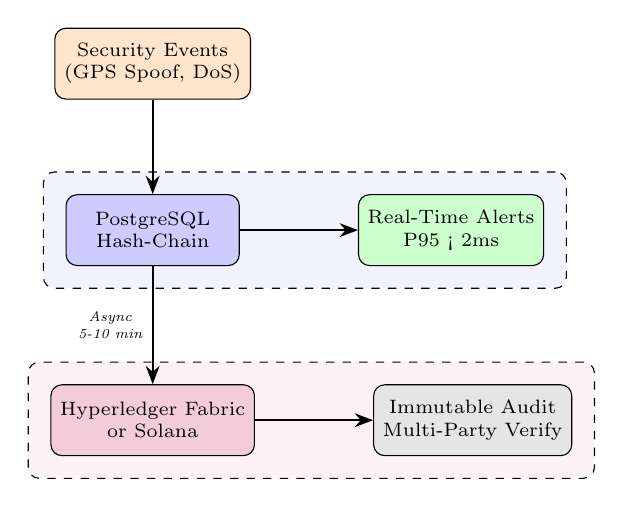
\begin{tikzpicture}[
    node distance=1.2cm,
    box/.style={rectangle, draw, rounded corners, minimum width=2.2cm, minimum height=0.9cm, align=center, font=\scriptsize},
    layer/.style={rectangle, draw, dashed, rounded corners, inner sep=8pt},
    arrow/.style={->, >=Stealth, thick},
    label/.style={font=\tiny\itshape, align=center}
]
% Security Events source
\node[box, fill=orange!20] (events) {Security Events\\(GPS Spoof, DoS)};

% Real-time layer
\node[box, fill=blue!20, below=of events] (postgres) {PostgreSQL\\Hash-Chain};
\node[box, fill=green!20, right=1.5cm of postgres] (alerts) {Real-Time Alerts\\P95 < 2ms};

% Audit layer
\node[box, fill=purple!20, below=1.5cm of postgres] (hyperledger) {Hyperledger Fabric\\or Solana};
\node[box, fill=gray!20, right=1.5cm of hyperledger] (audit) {Immutable Audit\\Multi-Party Verify};

% Arrows
\draw[arrow] (events) -- (postgres);
\draw[arrow] (postgres) -- (alerts);
\draw[arrow] (postgres) -- node[left, label] {Async\\5-10 min} (hyperledger);
\draw[arrow] (hyperledger) -- (audit);

% Layer labels
\begin{scope}[on background layer]
    \node[layer, fill=blue!5, fit=(postgres)(alerts), label={[anchor=north west, font=\scriptsize\bfseries]north west:Real-Time Layer}] {};
    \node[layer, fill=purple!5, fit=(hyperledger)(audit), label={[anchor=north west, font=\scriptsize\bfseries]north west:Audit Layer}] {};
\end{scope}
\end{tikzpicture}
\caption{Recommended Hybrid Architecture. Real-time events flow to PostgreSQL; periodic Merkle root anchors commit to blockchain for immutable audit.}
\label{fig:hybrid_architecture}
\end{figure}

\textbf{Real-Time Layer (PostgreSQL)}:
\begin{itemize}
\item Receives all security events with sub-2ms latency
\item Maintains hash-chained audit log for tamper detection
\item Supports 5,000+ TPS for fleet-scale operations
\item Triggers immediate alerts on attack detection
\end{itemize}

\textbf{Audit Layer (Hyperledger Fabric)}:
\begin{itemize}
\item Receives Merkle root anchors every 5--10 minutes
\item Provides distributed verification across stakeholders
\item Satisfies regulatory requirements for immutable records
\item Enables multi-party audit without central trust
\end{itemize}

This architecture provides real-time performance (1.39ms) while achieving blockchain's trust guarantees for audit purposes. The Merkle root anchoring approach reduces blockchain transaction volume by orders of magnitude while maintaining cryptographic linkage to the complete event history.

\subsection{Public vs Permissioned Blockchain}

For AAM applications, Hyperledger Fabric offers significant advantages over Solana:

\begin{table}[htbp]
\caption{Public vs Permissioned Comparison}
\label{tab:public_permissioned}
\centering
\begin{tabular}{lcc}
\toprule
\textbf{Factor} & \textbf{Solana} & \textbf{Hyperledger} \\
\midrule
Finality & 12.8s & $\sim$2s \\
Uptime & 99.94\% & Configurable \\
Participants & Unknown & Known/Accountable \\
Transaction Cost & $\sim$\$0.00025 & Free (private) \\
Regulatory Fit & Poor & Strong \\
\bottomrule
\end{tabular}
\end{table}

Aviation regulators (FAA, EASA) require known, accountable participants in safety-critical systems. Public blockchains with anonymous validators conflict with this requirement. Permissioned blockchain enables consortium governance where operators, regulators, and insurers maintain identified nodes.

\subsection{Limitations and Threats to Validity}

\textbf{Internal validity}: Local test environments do not replicate production network latency. Hyperledger CLI usage artificially limited throughput compared to SDK implementations. PostgreSQL ran single-node without replication overhead.

\textbf{External validity}: Results from processed datasets may differ from real-time attack detection in flight. The UAV dataset, while realistic, represents specific attack scenarios that may not cover all AAM threats.

\textbf{Construct validity}: We measured end-to-end latency including confirmation, which is appropriate for audit logging but may overstate overhead for fire-and-forget logging patterns.

Future work should evaluate: (1) production Hyperledger deployments across geographically distributed nodes, (2) Solana's Alpenglow consensus when available, (3) real-time attack detection latency during flight operations.

\section{Conclusion}
\label{sec:conclusion}

This paper presented the first quantitative evaluation of blockchain versus traditional databases for AAM security event logging. Using real UAV cyberattack datasets with 157,501 events across six attack types plus benign operations, we compared PostgreSQL (hash-chained), Hyperledger Fabric (permissioned blockchain), and Solana (public blockchain) across latency, throughput, and security dimensions.

Our findings confirm that blockchain cannot meet real-time requirements for AAM security alerting. PostgreSQL achieves 1.39ms P95 latency at 5,000 TPS, compared to 2,182ms for Hyperledger Fabric (1,570x slower) and 15,157ms for Solana (10,900x slower). All systems passed tamper detection and data integrity tests, confirming that the security guarantees are comparable.

The performance gap reflects fundamental architectural tradeoffs: blockchain consensus prioritizes consistency and distributed trust over latency. For multi-stakeholder AAM ecosystems requiring independent audit capabilities, this overhead may be acceptable for non-real-time use cases.

We recommend a hybrid architecture combining PostgreSQL for real-time operations (sub-2ms latency, 5,000+ TPS) with periodic Hyperledger Fabric anchoring for immutable audit trails. This approach provides the performance required for safety-critical systems while satisfying regulatory requirements for tamper-evident, multi-party verifiable logging.

All implementations---including Go chaincode, Rust/Anchor programs, PostgreSQL schema, load testing tools, and security test suites---are available in the accompanying repository for reproduction and extension.

\section*{Acknowledgment}

This work was conducted as part of the Intelligent DevOps of Large-Scale Software Systems course at Polytechnique Montreal. The UAV cyberattack dataset was provided by Hassler et al. under NSF Award 2220346.

\balance
\bibliographystyle{IEEEtran}
\bibliography{references}

\end{document}
